% !TEX root = main.tex
\section{Optimization and Characterisation of FID in water sample}
\label{sec:OptimizationandCharacterisationofFIDinwatersample}

One of the main goals of this experiment is to measure a good FID of the water sample. In order to do so we first have to optimize our FID signal of the water probe.\newline
At first the inhomogeneity of the magnetic field has to be cancelled. The process to make the magnetic field more homogeneous is to \textit{autoshim} the components of the gradient coil. The computer programm does this automatically. So it deshims the system step by step and checks if the output maximizes or minimizes. By checking many different combinations it finds the best shimming values for the gradient coil. In our case they are:
\begin{align*}
    x &= \SI{10.11}{\milli \ampere}\\
    y &= \SI{20.88}{\milli \ampere}\\
    z &= \SI{-20.07}{\milli \ampere} \ .
    \label{eq: shimmingvalues}
\end{align*}
That means with those shimming values the magnetic field in the setup is homogeneous.
\\
The second optimization step is to change the B$_1$ pulse duration. The longer the pulse duration is, the bigger is the angle of the flipping spins and thus the signal will get stronger (only for flipping angles till \SI{90}{\degree}). The best signal is obtained for an flipping angle of \SI{90}{\degree}, because with this angle the spins only have a component in the transversal plane and therefore the signal is maximized. If the pulse duration is too long, than the flipping angle is bigger than \SI{90}{\degree} and the spins get a horizontal component again and the signal will decrease again. When a flipping angle of \SI{180}{\degree} is reached the signal will be at its minimum. Afterwards the signal will raise again, because of the increasing horizontal component. Figure \ref{fig:B1dauer} shows this issue. The maxmimum at a pulse duration of \SI{1.35}{\milli \second} is clearly visible. This means that after apllying a B$_1$ pulse with a duration of \SI{1.35}{\milli \second} the spins are in the transversal plane and therefore the best signal is obtained.
\begin{figure}[H]
    \centering
    % GNUPLOT: LaTeX picture with Postscript
\begingroup
  % Encoding inside the plot.  In the header of your document, this encoding
  % should to defined, e.g., by using
  % \usepackage[cp1252,<other encodings>]{inputenc}
  \inputencoding{cp1252}%
  \makeatletter
  \providecommand\color[2][]{%
    \GenericError{(gnuplot) \space\space\space\@spaces}{%
      Package color not loaded in conjunction with
      terminal option `colourtext'%
    }{See the gnuplot documentation for explanation.%
    }{Either use 'blacktext' in gnuplot or load the package
      color.sty in LaTeX.}%
    \renewcommand\color[2][]{}%
  }%
  \providecommand\includegraphics[2][]{%
    \GenericError{(gnuplot) \space\space\space\@spaces}{%
      Package graphicx or graphics not loaded%
    }{See the gnuplot documentation for explanation.%
    }{The gnuplot epslatex terminal needs graphicx.sty or graphics.sty.}%
    \renewcommand\includegraphics[2][]{}%
  }%
  \providecommand\rotatebox[2]{#2}%
  \@ifundefined{ifGPcolor}{%
    \newif\ifGPcolor
    \GPcolorfalse
  }{}%
  \@ifundefined{ifGPblacktext}{%
    \newif\ifGPblacktext
    \GPblacktexttrue
  }{}%
  % define a \g@addto@macro without @ in the name:
  \let\gplgaddtomacro\g@addto@macro
  % define empty templates for all commands taking text:
  \gdef\gplbacktext{}%
  \gdef\gplfronttext{}%
  \makeatother
  \ifGPblacktext
    % no textcolor at all
    \def\colorrgb#1{}%
    \def\colorgray#1{}%
  \else
    % gray or color?
    \ifGPcolor
      \def\colorrgb#1{\color[rgb]{#1}}%
      \def\colorgray#1{\color[gray]{#1}}%
      \expandafter\def\csname LTw\endcsname{\color{white}}%
      \expandafter\def\csname LTb\endcsname{\color{black}}%
      \expandafter\def\csname LTa\endcsname{\color{black}}%
      \expandafter\def\csname LT0\endcsname{\color[rgb]{1,0,0}}%
      \expandafter\def\csname LT1\endcsname{\color[rgb]{0,1,0}}%
      \expandafter\def\csname LT2\endcsname{\color[rgb]{0,0,1}}%
      \expandafter\def\csname LT3\endcsname{\color[rgb]{1,0,1}}%
      \expandafter\def\csname LT4\endcsname{\color[rgb]{0,1,1}}%
      \expandafter\def\csname LT5\endcsname{\color[rgb]{1,1,0}}%
      \expandafter\def\csname LT6\endcsname{\color[rgb]{0,0,0}}%
      \expandafter\def\csname LT7\endcsname{\color[rgb]{1,0.3,0}}%
      \expandafter\def\csname LT8\endcsname{\color[rgb]{0.5,0.5,0.5}}%
    \else
      % gray
      \def\colorrgb#1{\color{black}}%
      \def\colorgray#1{\color[gray]{#1}}%
      \expandafter\def\csname LTw\endcsname{\color{white}}%
      \expandafter\def\csname LTb\endcsname{\color{black}}%
      \expandafter\def\csname LTa\endcsname{\color{black}}%
      \expandafter\def\csname LT0\endcsname{\color{black}}%
      \expandafter\def\csname LT1\endcsname{\color{black}}%
      \expandafter\def\csname LT2\endcsname{\color{black}}%
      \expandafter\def\csname LT3\endcsname{\color{black}}%
      \expandafter\def\csname LT4\endcsname{\color{black}}%
      \expandafter\def\csname LT5\endcsname{\color{black}}%
      \expandafter\def\csname LT6\endcsname{\color{black}}%
      \expandafter\def\csname LT7\endcsname{\color{black}}%
      \expandafter\def\csname LT8\endcsname{\color{black}}%
    \fi
  \fi
    \setlength{\unitlength}{0.0500bp}%
    \ifx\gptboxheight\undefined%
      \newlength{\gptboxheight}%
      \newlength{\gptboxwidth}%
      \newsavebox{\gptboxtext}%
    \fi%
    \setlength{\fboxrule}{0.5pt}%
    \setlength{\fboxsep}{1pt}%
\begin{picture}(7200.00,5040.00)%
    \gplgaddtomacro\gplbacktext{%
      \csname LTb\endcsname%%
      \put(814,704){\makebox(0,0)[r]{\strut{}$60$}}%
      \put(814,1527){\makebox(0,0)[r]{\strut{}$80$}}%
      \put(814,2350){\makebox(0,0)[r]{\strut{}$100$}}%
      \put(814,3173){\makebox(0,0)[r]{\strut{}$120$}}%
      \put(814,3996){\makebox(0,0)[r]{\strut{}$140$}}%
      \put(814,4819){\makebox(0,0)[r]{\strut{}$160$}}%
      \put(946,484){\makebox(0,0){\strut{}$0$}}%
      \put(1678,484){\makebox(0,0){\strut{}$0.5$}}%
      \put(2410,484){\makebox(0,0){\strut{}$1$}}%
      \put(3142,484){\makebox(0,0){\strut{}$1.5$}}%
      \put(3875,484){\makebox(0,0){\strut{}$2$}}%
      \put(4607,484){\makebox(0,0){\strut{}$2.5$}}%
      \put(5339,484){\makebox(0,0){\strut{}$3$}}%
      \put(6071,484){\makebox(0,0){\strut{}$3.5$}}%
      \put(6803,484){\makebox(0,0){\strut{}$4$}}%
    }%
    \gplgaddtomacro\gplfronttext{%
      \csname LTb\endcsname%%
      \put(209,2761){\rotatebox{-270}{\makebox(0,0){\strut{}FID amplitude}}}%
      \put(3874,154){\makebox(0,0){\strut{}$B_1$ pulse in $\si{}{ms}$}}%
      \csname LTb\endcsname%%
      \put(5816,4646){\makebox(0,0)[r]{\strut{}measured resonance amplitude}}%
    }%
    \gplbacktext
    \put(0,0){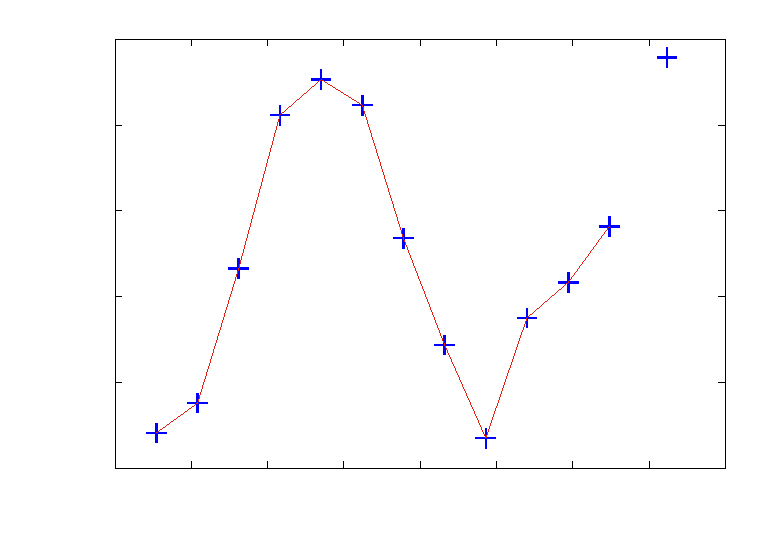
\includegraphics{plots/B1dauer}}%
    \gplfronttext
  \end{picture}%
\endgroup

    \caption[This figure shows which impact the B$_1$ pulse duration has to the ampitude of the FID.]{This figure shows which impact the B$_1$ pulse duration has to the ampitude of the FID. It is clearly visible that the duration has a maximum at \SI{1.35}{\milli \second} which is the duration for a \SI{90}{\degree} pulse.}
    \label{fig:B1dauer}
\end{figure}
Figure \ref{fig:pulsedurationbeispiel} exemplarily shows the correlation of the B$_1$ pulse duration and the signal which the coil detects. It is clearly visible that the amplitude is better for the pulse duration of \SI{1.35}{\milli \second} than for the pulse duration of \SI{0.27}{\milli \second}. The signal that was taken for the pulse duration of \SI{0.27}{\milli \second} is at the minimum of the figure \ref{fig:B1dauer} and therefore it is correct that the amplitude of the spectrum with the pulse duration of \SI{1.35}{\milli \second} is higher.
\begin{figure}[H]
    \centering
    % GNUPLOT: LaTeX picture with Postscript
\begingroup
  % Encoding inside the plot.  In the header of your document, this encoding
  % should to defined, e.g., by using
  % \usepackage[cp1252,<other encodings>]{inputenc}
  \inputencoding{cp1252}%
  \makeatletter
  \providecommand\color[2][]{%
    \GenericError{(gnuplot) \space\space\space\@spaces}{%
      Package color not loaded in conjunction with
      terminal option `colourtext'%
    }{See the gnuplot documentation for explanation.%
    }{Either use 'blacktext' in gnuplot or load the package
      color.sty in LaTeX.}%
    \renewcommand\color[2][]{}%
  }%
  \providecommand\includegraphics[2][]{%
    \GenericError{(gnuplot) \space\space\space\@spaces}{%
      Package graphicx or graphics not loaded%
    }{See the gnuplot documentation for explanation.%
    }{The gnuplot epslatex terminal needs graphicx.sty or graphics.sty.}%
    \renewcommand\includegraphics[2][]{}%
  }%
  \providecommand\rotatebox[2]{#2}%
  \@ifundefined{ifGPcolor}{%
    \newif\ifGPcolor
    \GPcolorfalse
  }{}%
  \@ifundefined{ifGPblacktext}{%
    \newif\ifGPblacktext
    \GPblacktexttrue
  }{}%
  % define a \g@addto@macro without @ in the name:
  \let\gplgaddtomacro\g@addto@macro
  % define empty templates for all commands taking text:
  \gdef\gplbacktext{}%
  \gdef\gplfronttext{}%
  \makeatother
  \ifGPblacktext
    % no textcolor at all
    \def\colorrgb#1{}%
    \def\colorgray#1{}%
  \else
    % gray or color?
    \ifGPcolor
      \def\colorrgb#1{\color[rgb]{#1}}%
      \def\colorgray#1{\color[gray]{#1}}%
      \expandafter\def\csname LTw\endcsname{\color{white}}%
      \expandafter\def\csname LTb\endcsname{\color{black}}%
      \expandafter\def\csname LTa\endcsname{\color{black}}%
      \expandafter\def\csname LT0\endcsname{\color[rgb]{1,0,0}}%
      \expandafter\def\csname LT1\endcsname{\color[rgb]{0,1,0}}%
      \expandafter\def\csname LT2\endcsname{\color[rgb]{0,0,1}}%
      \expandafter\def\csname LT3\endcsname{\color[rgb]{1,0,1}}%
      \expandafter\def\csname LT4\endcsname{\color[rgb]{0,1,1}}%
      \expandafter\def\csname LT5\endcsname{\color[rgb]{1,1,0}}%
      \expandafter\def\csname LT6\endcsname{\color[rgb]{0,0,0}}%
      \expandafter\def\csname LT7\endcsname{\color[rgb]{1,0.3,0}}%
      \expandafter\def\csname LT8\endcsname{\color[rgb]{0.5,0.5,0.5}}%
    \else
      % gray
      \def\colorrgb#1{\color{black}}%
      \def\colorgray#1{\color[gray]{#1}}%
      \expandafter\def\csname LTw\endcsname{\color{white}}%
      \expandafter\def\csname LTb\endcsname{\color{black}}%
      \expandafter\def\csname LTa\endcsname{\color{black}}%
      \expandafter\def\csname LT0\endcsname{\color{black}}%
      \expandafter\def\csname LT1\endcsname{\color{black}}%
      \expandafter\def\csname LT2\endcsname{\color{black}}%
      \expandafter\def\csname LT3\endcsname{\color{black}}%
      \expandafter\def\csname LT4\endcsname{\color{black}}%
      \expandafter\def\csname LT5\endcsname{\color{black}}%
      \expandafter\def\csname LT6\endcsname{\color{black}}%
      \expandafter\def\csname LT7\endcsname{\color{black}}%
      \expandafter\def\csname LT8\endcsname{\color{black}}%
    \fi
  \fi
    \setlength{\unitlength}{0.0500bp}%
    \ifx\gptboxheight\undefined%
      \newlength{\gptboxheight}%
      \newlength{\gptboxwidth}%
      \newsavebox{\gptboxtext}%
    \fi%
    \setlength{\fboxrule}{0.5pt}%
    \setlength{\fboxsep}{1pt}%
\begin{picture}(7200.00,5040.00)%
    \gplgaddtomacro\gplbacktext{%
      \csname LTb\endcsname%%
      \put(682,704){\makebox(0,0)[r]{\strut{}$0$}}%
      \put(682,1161){\makebox(0,0)[r]{\strut{}$10$}}%
      \put(682,1618){\makebox(0,0)[r]{\strut{}$20$}}%
      \put(682,2076){\makebox(0,0)[r]{\strut{}$30$}}%
      \put(682,2533){\makebox(0,0)[r]{\strut{}$40$}}%
      \put(682,2990){\makebox(0,0)[r]{\strut{}$50$}}%
      \put(682,3447){\makebox(0,0)[r]{\strut{}$60$}}%
      \put(682,3905){\makebox(0,0)[r]{\strut{}$70$}}%
      \put(682,4362){\makebox(0,0)[r]{\strut{}$80$}}%
      \put(682,4819){\makebox(0,0)[r]{\strut{}$90$}}%
      \put(814,484){\makebox(0,0){\strut{}$1800$}}%
      \put(2012,484){\makebox(0,0){\strut{}$1820$}}%
      \put(3210,484){\makebox(0,0){\strut{}$1840$}}%
      \put(4407,484){\makebox(0,0){\strut{}$1860$}}%
      \put(5605,484){\makebox(0,0){\strut{}$1880$}}%
      \put(6803,484){\makebox(0,0){\strut{}$1900$}}%
    }%
    \gplgaddtomacro\gplfronttext{%
      \csname LTb\endcsname%%
      \put(209,2761){\rotatebox{-270}{\makebox(0,0){\strut{}Amplitude in $\si{\mu \volt}$}}}%
      \put(3808,154){\makebox(0,0){\strut{}Frequency in $\si{\hertz}$}}%
      \csname LTb\endcsname%%
      \put(5816,4646){\makebox(0,0)[r]{\strut{}$\SI{0.27}{\milli \second}$ B$_1$ duration}}%
      \csname LTb\endcsname%%
      \put(5816,4426){\makebox(0,0)[r]{\strut{}$\SI{1.35}{\milli \second}$ B$_1$ duration}}%
    }%
    \gplbacktext
    \put(0,0){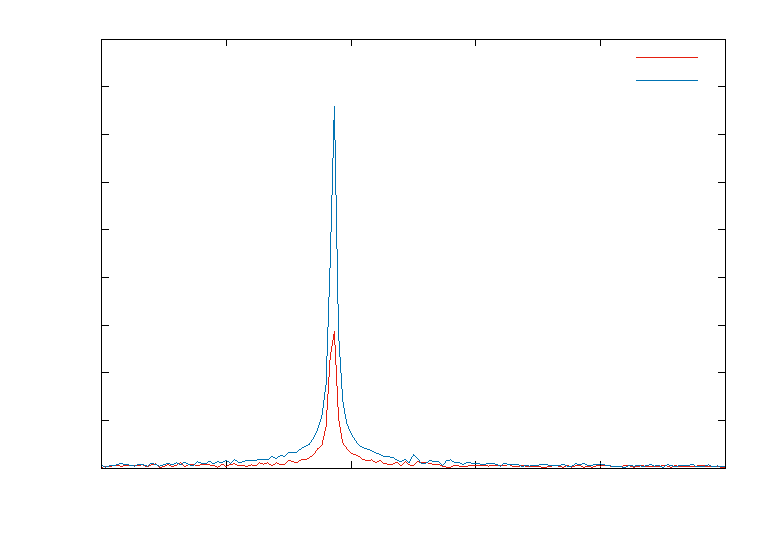
\includegraphics{plots/138_puls_and_collect_number_of_delay25ms_Pulseduration0_27ms}}%
    \gplfronttext
  \end{picture}%
\endgroup

    \caption[Example spectrum for two different B$_1$ pulse durations.]{Example spectrum for two different B$_1$ pulse durations. The peak which is higher corresponds to the \SI{1.35}{\milli \second} duration pulse and represents the \SI{90}{\degree} pulse. This peak is high, because at this duration most of the spins are in the transversal plane and therfore the amplitude is maximal.}
    \label{fig:pulsedurationbeispiel}
\end{figure}
Now that the B$_1$ pulse duration is also optimized, we can have a closer look at the capacity of the LCR circuit of the B$_1$ coil again. First it is necessary to know that the B$_1$ pulse is applied by a \textit{rectangular} function and the fourie transformation of a \textit{rectangular} function is a \textit{sinc} function. Therefore the fourier ransformed spectrum of the B$_1$ pulse signal is a \textit{sinc} function. When we measure the signal shortly (acquisition delay: \SI{2}{\milli \second}) after the \SI{90}{\degree} pulse, there shoud be a \textit{sinc} function visible and indeed this is what we obtained (figure \ref{fig:Pulsandcollect}). In figure \ref{fig:Pulsandcollect} there is also a really sharp peak visible. This is referd to the hydrogen signal. The hydrogen signal is independed of the applied capacity, but the $B_1$ pulse is, because the capacity changes the properties of the LCR-circuit of the B$_1$ coil. The best capacity is adjusted when the hydrogen signal is in the middle of the \textit{sinc} function, because then the LCR-circuit is tuned to the lamor frequency of the hydrogen signal. This is also visible by the amplitude of the spectrum in figure \ref{fig:Pulsandcollect}. The amplitude of the spectrum which was observed for a capacity of \SI{13.8}{\nano \farad} is higher than for the amplitude of the spectrum which was observed for a capacity of \SI{14.2}{\nano \farad}. As already explained before in the chapter \ref{sec:CoilAnalyssis} the capacity of \SI{13.8}{\nano \farad} is indeed the best capacity in order to observe a maximized spectrum.
\begin{figure}[H]
    \centering
    % GNUPLOT: LaTeX picture with Postscript
\begingroup
  % Encoding inside the plot.  In the header of your document, this encoding
  % should to defined, e.g., by using
  % \usepackage[cp1252,<other encodings>]{inputenc}
  \inputencoding{cp1252}%
  \makeatletter
  \providecommand\color[2][]{%
    \GenericError{(gnuplot) \space\space\space\@spaces}{%
      Package color not loaded in conjunction with
      terminal option `colourtext'%
    }{See the gnuplot documentation for explanation.%
    }{Either use 'blacktext' in gnuplot or load the package
      color.sty in LaTeX.}%
    \renewcommand\color[2][]{}%
  }%
  \providecommand\includegraphics[2][]{%
    \GenericError{(gnuplot) \space\space\space\@spaces}{%
      Package graphicx or graphics not loaded%
    }{See the gnuplot documentation for explanation.%
    }{The gnuplot epslatex terminal needs graphicx.sty or graphics.sty.}%
    \renewcommand\includegraphics[2][]{}%
  }%
  \providecommand\rotatebox[2]{#2}%
  \@ifundefined{ifGPcolor}{%
    \newif\ifGPcolor
    \GPcolorfalse
  }{}%
  \@ifundefined{ifGPblacktext}{%
    \newif\ifGPblacktext
    \GPblacktexttrue
  }{}%
  % define a \g@addto@macro without @ in the name:
  \let\gplgaddtomacro\g@addto@macro
  % define empty templates for all commands taking text:
  \gdef\gplbacktext{}%
  \gdef\gplfronttext{}%
  \makeatother
  \ifGPblacktext
    % no textcolor at all
    \def\colorrgb#1{}%
    \def\colorgray#1{}%
  \else
    % gray or color?
    \ifGPcolor
      \def\colorrgb#1{\color[rgb]{#1}}%
      \def\colorgray#1{\color[gray]{#1}}%
      \expandafter\def\csname LTw\endcsname{\color{white}}%
      \expandafter\def\csname LTb\endcsname{\color{black}}%
      \expandafter\def\csname LTa\endcsname{\color{black}}%
      \expandafter\def\csname LT0\endcsname{\color[rgb]{1,0,0}}%
      \expandafter\def\csname LT1\endcsname{\color[rgb]{0,1,0}}%
      \expandafter\def\csname LT2\endcsname{\color[rgb]{0,0,1}}%
      \expandafter\def\csname LT3\endcsname{\color[rgb]{1,0,1}}%
      \expandafter\def\csname LT4\endcsname{\color[rgb]{0,1,1}}%
      \expandafter\def\csname LT5\endcsname{\color[rgb]{1,1,0}}%
      \expandafter\def\csname LT6\endcsname{\color[rgb]{0,0,0}}%
      \expandafter\def\csname LT7\endcsname{\color[rgb]{1,0.3,0}}%
      \expandafter\def\csname LT8\endcsname{\color[rgb]{0.5,0.5,0.5}}%
    \else
      % gray
      \def\colorrgb#1{\color{black}}%
      \def\colorgray#1{\color[gray]{#1}}%
      \expandafter\def\csname LTw\endcsname{\color{white}}%
      \expandafter\def\csname LTb\endcsname{\color{black}}%
      \expandafter\def\csname LTa\endcsname{\color{black}}%
      \expandafter\def\csname LT0\endcsname{\color{black}}%
      \expandafter\def\csname LT1\endcsname{\color{black}}%
      \expandafter\def\csname LT2\endcsname{\color{black}}%
      \expandafter\def\csname LT3\endcsname{\color{black}}%
      \expandafter\def\csname LT4\endcsname{\color{black}}%
      \expandafter\def\csname LT5\endcsname{\color{black}}%
      \expandafter\def\csname LT6\endcsname{\color{black}}%
      \expandafter\def\csname LT7\endcsname{\color{black}}%
      \expandafter\def\csname LT8\endcsname{\color{black}}%
    \fi
  \fi
    \setlength{\unitlength}{0.0500bp}%
    \ifx\gptboxheight\undefined%
      \newlength{\gptboxheight}%
      \newlength{\gptboxwidth}%
      \newsavebox{\gptboxtext}%
    \fi%
    \setlength{\fboxrule}{0.5pt}%
    \setlength{\fboxsep}{1pt}%
\begin{picture}(7200.00,5040.00)%
    \gplgaddtomacro\gplbacktext{%
      \csname LTb\endcsname%%
      \put(814,704){\makebox(0,0)[r]{\strut{}$0$}}%
      \put(814,1390){\makebox(0,0)[r]{\strut{}$20$}}%
      \put(814,2076){\makebox(0,0)[r]{\strut{}$40$}}%
      \put(814,2762){\makebox(0,0)[r]{\strut{}$60$}}%
      \put(814,3447){\makebox(0,0)[r]{\strut{}$80$}}%
      \put(814,4133){\makebox(0,0)[r]{\strut{}$100$}}%
      \put(814,4819){\makebox(0,0)[r]{\strut{}$120$}}%
      \put(946,484){\makebox(0,0){\strut{}$1650$}}%
      \put(1678,484){\makebox(0,0){\strut{}$1700$}}%
      \put(2410,484){\makebox(0,0){\strut{}$1750$}}%
      \put(3142,484){\makebox(0,0){\strut{}$1800$}}%
      \put(3875,484){\makebox(0,0){\strut{}$1850$}}%
      \put(4607,484){\makebox(0,0){\strut{}$1900$}}%
      \put(5339,484){\makebox(0,0){\strut{}$1950$}}%
      \put(6071,484){\makebox(0,0){\strut{}$2000$}}%
      \put(6803,484){\makebox(0,0){\strut{}$2050$}}%
    }%
    \gplgaddtomacro\gplfronttext{%
      \csname LTb\endcsname%%
      \put(209,2761){\rotatebox{-270}{\makebox(0,0){\strut{}Amplitude}}}%
      \put(3874,154){\makebox(0,0){\strut{}Frequency in $\si{\hertz}$}}%
      \csname LTb\endcsname%%
      \put(5816,4646){\makebox(0,0)[r]{\strut{}capacity $\SI{13.8}{\nano \farad}$}}%
      \csname LTb\endcsname%%
      \put(5816,4426){\makebox(0,0)[r]{\strut{}capacity $\SI{14.2}{\nano \farad}$}}%
    }%
    \gplbacktext
    \put(0,0){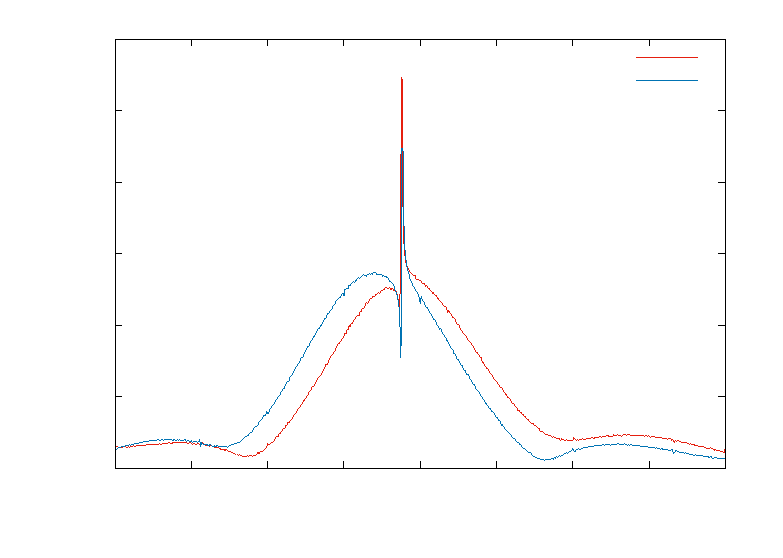
\includegraphics{plots/Pulsandcollect138}}%
    \gplfronttext
  \end{picture}%
\endgroup

    \caption[This figure shows the impact of the capacity in the LCR circuit of the B$_1$ coil.]{This figure shows the impact of the capacity in the LCR circuit of the B$_1$ coil. The \textit{sinc} function comes from the fourier transformed B$_1$ pulse, which is rectangular. The peak at \SI{1837.27 \pm 0.05}{\hertz} is the peak from the hydrogen signal.}
    \label{fig:Pulsandcollect}
\end{figure}
Now that the FID signal is optimized best we can start to characterize it. Therefore we measure a FID with a acquisition delay of \SI{25}{\milli \second}, because after this delay there are no effects from the rectangular applied B$_1$ pulse anymore (no \textit{sinc} function in the spectrum). The figure \ref{fig:Pulsandcollect138_delay_25_gauss} shows the observed spectrum and two different fit possibilities.\newline
One option to fit a peak in a spectrum is by applying a \textit{voigt}-profile ($V(x;\sigma , \gamma)$). This function is a convolution of the \textit{Cauchy-Lorentz}- and \textit{Gaussian}-distribution and is described by following formula:
\begin{align}
    V(x;\sigma , \gamma) &= ( G \star L)(x) = \int G(\tau) L(x-\tau) d\tau \\
    G(x;\sigma) &= \frac{exp\left(\frac{-x^2}{2\sigma^2}\right)}{\sigma \sqrt{2 \pi}} \\
    L(x;\gamma)  &= \frac{\gamma}{\pi \left( x^2+\gamma^2\right)} \ .
    \label{eq: voigt} 
\end{align}
$\sigma$ represents the standard deviation, $\gamma$ is half of the peak width at half height from the \textit{Lorentz}-distribution and $x$ is the shift from the line center. In figure \ref{fig:Pulsandcollect138_delay_25_gauss} the \textit{voigt}-profile (green) is fitted to the measured spectrum (red). The problem about this fit is that is not as sharp as the measured data. This might be, due to the fact that the measured spectrum does not have many data points especially around the maximum. Therefore the peak is really sharp and a correct fit with the \textit{voigt}-profile is rather difficult. Therefore a second fit function has been apllied. This time only the \textit{Gaussian}-distribution. This fit function is better to calculate the width of the peak, due to the fact that it is easier to fit it to this narrow peak. The full width of the peak at have maximum (FWHM) is calculated by the applied \textit{Gaussian}-fit and is \SI{1.177 \pm 0.042}{\hertz}. \newline
The amplitude of the peak is \SI{73.85}{\mu \volt} according to the \textit{Gaussian}-fit and is in comparison to the amplitude of the noise measurement (magnitude \SI{1}{}) in figure \ref{fig: MonitorNoise138} rather high. The signal to noise ratio of this point is \SI{47.57}{}. To calculate this value the amplitude at \SI{1837.27}{\hertz} (center of the peak) in figure \ref{fig:Pulsandcollect138_delay_25_gauss} is devided by the value of the amplitude at the same frequency in figure \ref{fig: MonitorNoise138}. That value clearly shows that the peak must come from the hydrogen signal and is barely disturbed by any noise.\newline
The width of the measured hydrogen peak at half hight (FWHM) is \SI{1.177 \pm 0.042}{\hertz} and therefore really sharp. An even better value can only be achieved by tuning the setup even more. To show the physical properties, this value is though of a really good size.\newline
The disadvantage of the \textit{Gaussian}-fit is that area under the curve does not equal the measured one, especially around \SI{1836}{\hertz} and \SI{1839}{\hertz}. Therefore the discussion about the integral under the measured curve will just be qualitative and will be done in the chapter \ref{sec:Hahnecho}.\newline
It is also possible to take a measurement of the imaginary signal of the peak in figure \ref{fig:Pulsandcollect138_delay_25_gauss}. Unfortunately we did not safe this data. Therefore we explain what we should see and what it means. The imaginary component discribes the dispersion spectrum. The spectrum then has to look like kind of a hyperbolic function with the pole exactly at \SI{1837.27}{\hertz} (center of the peak). Since it is no real hyperbolic function there exist values at the pole. Those values are aligned in a vertical line.
\begin{figure}[H]
    \centering
    % GNUPLOT: LaTeX picture with Postscript
\begingroup
  % Encoding inside the plot.  In the header of your document, this encoding
  % should to defined, e.g., by using
  % \usepackage[cp1252,<other encodings>]{inputenc}
  \inputencoding{cp1252}%
  \makeatletter
  \providecommand\color[2][]{%
    \GenericError{(gnuplot) \space\space\space\@spaces}{%
      Package color not loaded in conjunction with
      terminal option `colourtext'%
    }{See the gnuplot documentation for explanation.%
    }{Either use 'blacktext' in gnuplot or load the package
      color.sty in LaTeX.}%
    \renewcommand\color[2][]{}%
  }%
  \providecommand\includegraphics[2][]{%
    \GenericError{(gnuplot) \space\space\space\@spaces}{%
      Package graphicx or graphics not loaded%
    }{See the gnuplot documentation for explanation.%
    }{The gnuplot epslatex terminal needs graphicx.sty or graphics.sty.}%
    \renewcommand\includegraphics[2][]{}%
  }%
  \providecommand\rotatebox[2]{#2}%
  \@ifundefined{ifGPcolor}{%
    \newif\ifGPcolor
    \GPcolorfalse
  }{}%
  \@ifundefined{ifGPblacktext}{%
    \newif\ifGPblacktext
    \GPblacktexttrue
  }{}%
  % define a \g@addto@macro without @ in the name:
  \let\gplgaddtomacro\g@addto@macro
  % define empty templates for all commands taking text:
  \gdef\gplbacktext{}%
  \gdef\gplfronttext{}%
  \makeatother
  \ifGPblacktext
    % no textcolor at all
    \def\colorrgb#1{}%
    \def\colorgray#1{}%
  \else
    % gray or color?
    \ifGPcolor
      \def\colorrgb#1{\color[rgb]{#1}}%
      \def\colorgray#1{\color[gray]{#1}}%
      \expandafter\def\csname LTw\endcsname{\color{white}}%
      \expandafter\def\csname LTb\endcsname{\color{black}}%
      \expandafter\def\csname LTa\endcsname{\color{black}}%
      \expandafter\def\csname LT0\endcsname{\color[rgb]{1,0,0}}%
      \expandafter\def\csname LT1\endcsname{\color[rgb]{0,1,0}}%
      \expandafter\def\csname LT2\endcsname{\color[rgb]{0,0,1}}%
      \expandafter\def\csname LT3\endcsname{\color[rgb]{1,0,1}}%
      \expandafter\def\csname LT4\endcsname{\color[rgb]{0,1,1}}%
      \expandafter\def\csname LT5\endcsname{\color[rgb]{1,1,0}}%
      \expandafter\def\csname LT6\endcsname{\color[rgb]{0,0,0}}%
      \expandafter\def\csname LT7\endcsname{\color[rgb]{1,0.3,0}}%
      \expandafter\def\csname LT8\endcsname{\color[rgb]{0.5,0.5,0.5}}%
    \else
      % gray
      \def\colorrgb#1{\color{black}}%
      \def\colorgray#1{\color[gray]{#1}}%
      \expandafter\def\csname LTw\endcsname{\color{white}}%
      \expandafter\def\csname LTb\endcsname{\color{black}}%
      \expandafter\def\csname LTa\endcsname{\color{black}}%
      \expandafter\def\csname LT0\endcsname{\color{black}}%
      \expandafter\def\csname LT1\endcsname{\color{black}}%
      \expandafter\def\csname LT2\endcsname{\color{black}}%
      \expandafter\def\csname LT3\endcsname{\color{black}}%
      \expandafter\def\csname LT4\endcsname{\color{black}}%
      \expandafter\def\csname LT5\endcsname{\color{black}}%
      \expandafter\def\csname LT6\endcsname{\color{black}}%
      \expandafter\def\csname LT7\endcsname{\color{black}}%
      \expandafter\def\csname LT8\endcsname{\color{black}}%
    \fi
  \fi
    \setlength{\unitlength}{0.0500bp}%
    \ifx\gptboxheight\undefined%
      \newlength{\gptboxheight}%
      \newlength{\gptboxwidth}%
      \newsavebox{\gptboxtext}%
    \fi%
    \setlength{\fboxrule}{0.5pt}%
    \setlength{\fboxsep}{1pt}%
\begin{picture}(7200.00,5040.00)%
    \gplgaddtomacro\gplbacktext{%
      \csname LTb\endcsname%%
      \put(682,704){\makebox(0,0)[r]{\strut{}$0$}}%
      \put(682,1161){\makebox(0,0)[r]{\strut{}$10$}}%
      \put(682,1618){\makebox(0,0)[r]{\strut{}$20$}}%
      \put(682,2076){\makebox(0,0)[r]{\strut{}$30$}}%
      \put(682,2533){\makebox(0,0)[r]{\strut{}$40$}}%
      \put(682,2990){\makebox(0,0)[r]{\strut{}$50$}}%
      \put(682,3447){\makebox(0,0)[r]{\strut{}$60$}}%
      \put(682,3905){\makebox(0,0)[r]{\strut{}$70$}}%
      \put(682,4362){\makebox(0,0)[r]{\strut{}$80$}}%
      \put(682,4819){\makebox(0,0)[r]{\strut{}$90$}}%
      \put(814,484){\makebox(0,0){\strut{}$1830$}}%
      \put(1613,484){\makebox(0,0){\strut{}$1832$}}%
      \put(2411,484){\makebox(0,0){\strut{}$1834$}}%
      \put(3210,484){\makebox(0,0){\strut{}$1836$}}%
      \put(4008,484){\makebox(0,0){\strut{}$1838$}}%
      \put(4807,484){\makebox(0,0){\strut{}$1840$}}%
      \put(5605,484){\makebox(0,0){\strut{}$1842$}}%
      \put(6404,484){\makebox(0,0){\strut{}$1844$}}%
      \put(4208,2304){\makebox(0,0)[l]{\strut{}FWHM $= \SI{1.177 \pm 0.042}{\hertz}$}}%
      \put(4208,2762){\makebox(0,0)[l]{\strut{}$\sigma =  \SI{0.500 \pm 0.018}{\hertz}$}}%
    }%
    \gplgaddtomacro\gplfronttext{%
      \csname LTb\endcsname%%
      \put(209,2761){\rotatebox{-270}{\makebox(0,0){\strut{}Amplitude in $\si{\mu \volt}$}}}%
      \put(3808,154){\makebox(0,0){\strut{}Frequency in $\si{\hertz}$}}%
      \csname LTb\endcsname%%
      \put(5816,4646){\makebox(0,0)[r]{\strut{}magnitude spectrum}}%
      \csname LTb\endcsname%%
      \put(5816,4426){\makebox(0,0)[r]{\strut{}voigt-profile}}%
      \csname LTb\endcsname%%
      \put(5816,4206){\makebox(0,0)[r]{\strut{}\textsc{Gauss}-Fit}}%
    }%
    \gplbacktext
    \put(0,0){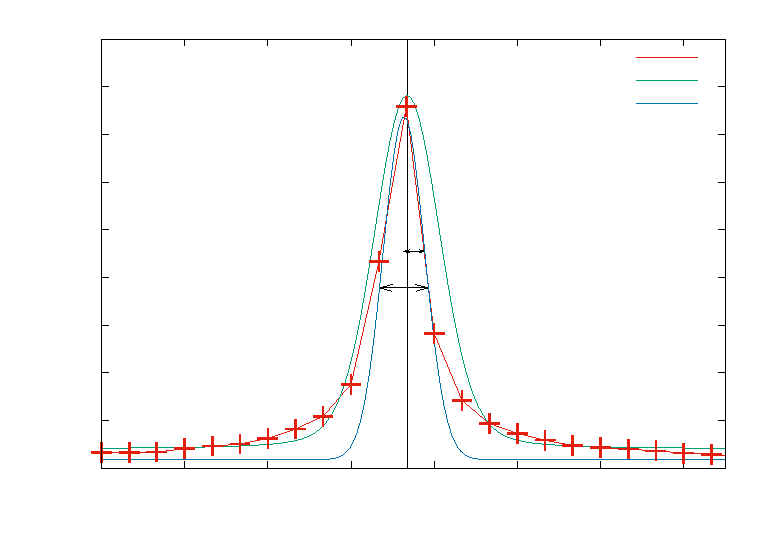
\includegraphics{plots/Pulsandcollect138_delay_25_gauss}}%
    \gplfronttext
  \end{picture}%
\endgroup

    \caption[This figure shows the measured hydrogen signal after an acquisition delay of \SI{25}{\milli \second} and two possible ways to fit the peak.]{This figure shows the measured hydrogen signal after an acquisition delay of \SI{25}{\milli \second} and two possible ways to fit the peak. Due to a very short frequency range the peak looks very wide. Indeed it is actually very sharp. To fit the peak a \textit{voigt}-profile and \textit{Gaussian}-fit is used.}
    \label{fig:Pulsandcollect138_delay_25_gauss}
\end{figure}